Uno strumento di misura ha una accuratezza di $10^{-6}$ (in opportune unità di misura). I dati misurati nelle posizioni $x_\mathrm{i}$ sono dati da $y_\mathrm{i}$, come descritto
dalla seguente tabella:
\begin{table}[H]
	\centering
	\begin{tabular}{|c|c|c|}
		\hline
		$i$ & $x_\mathrm{i}$ & $y_\mathrm{i}$ \\
		\hline
		$0$ & $0.010$ & $1.003626$ \\
		$1$ & $0.098$ & $1.025686$ \\
		$2$ & $0.127$ & $1.029512$ \\
		$3$ & $0.278$ & $1.029130$ \\
		$4$ & $0.547$ & $0.994781$ \\
		$5$ & $0.632$ & $0.990156$ \\
		$6$ & $0.815$ & $1.016687$ \\
		$7$ & $0.906$ & $1.057382$ \\
		$8$ & $0.913$ & $1.061462$ \\
		$9$ & $0.958$ & $1.091263$ \\
		$10$ & $0.965$ & $1.096476$ \\
		\hline
	\end{tabular}
\end{table}
Calcolare il grado minimo, ed i relativi coefficienti, del polinomio che meglio approssima i precedenti dati nel senso dei minimi quadrati con una adeguata accuratezza.
Graficare convenientemente i risultati ottenuti.

\hspace*{\fill}
\par\noindent\rule{\textwidth}{0.4pt}
\hspace*{\fill}

\textbf{Approssimazione polinomiale ai minimi quadrati}:
\lstinputlisting[language=Matlab]{Chapter-4/Exercise-21/lstsquare.m}
\begin{minipage}{\textwidth}
	\begin{lstlisting}[language=Matlab, caption=Codice Matlab]
	xi = [0.010; 0.098; 0.127; 0.278; 0.547; 0.632; 0.815; 0.906; 0.913; 0.958; 0.965];
	fi = [1.003626; 1.025686; 1.029512; 1.029130; 0.994781; 0.990156; 1.016687; 1.057382; 1.061462; 1.091263; 1.096476];
	a = 0;
	b = 2;
	x = linspace(a, b, 10001);
	n = length(xi);
	tol = 1E-6;
	[A, a, d] = lstsquare(xi, fi, tol);

	for m = 1 : n - 1
		p = polyval(A(1 : m, m), x);
		plot(x, p)
		hold on
	end
	legend('1', '2', '3', '4', '5', '6', '7', '8', '9', '10')
	hold off
	\end{lstlisting}
\end{minipage}

La seguente figura mostra l'approssimazione polinomiale ai minimi quadrati, al variare del grado $n$ del polinomio interpolante ($=1,2,3,4...10$):
\begin{figure}[H]
	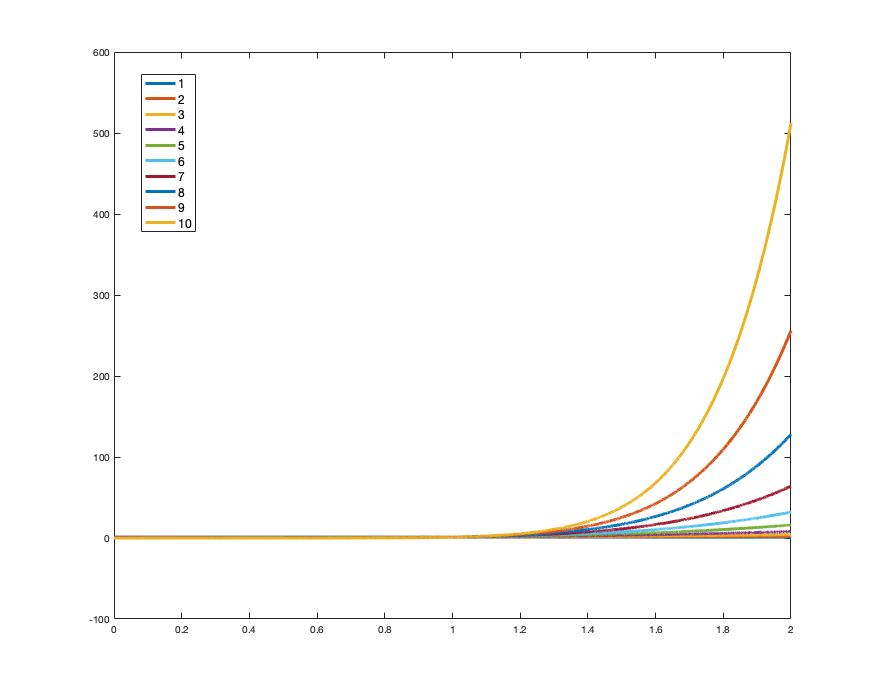
\includegraphics[width=\textwidth]{Chapter-4/Exercise-21/plot.jpg}
	\caption*{Approssimazione polinomiale ai minimi quadrati, con grado $n=1,2,3,4...10$ del polinomio interpolante}
\end{figure}
In particolare, è possibile osservare che l'approssimazione migliore di grado minimo che rispetta l'accuratezza prefissata, pari a $10^{-6}$, è data dal polinomio interpolante di grado $n = 4$, con i seguenti coefficienti, rappresentati sotto forma tabellare a partire dal peso relativo al termine noto del polinomio:
\begin{table}[H]
	\centering
	\begin{tabular}{|c|c|c|}
		\hline
		$i$ & $a_\mathrm{i}$ \\
		\hline
		$0$ & $9.999998544795017e-01$ \\
		$1$ & $3.750011620458070e-01$ \\
		$2$ & $-1.250002941638535e+00$ \\
		$3$ & $1.000001891005298e+00$ \\
		\hline
	\end{tabular}
\end{table}
